\documentclass[12pt,UTF8,a4paper]{ctexart}
\usepackage[margin=2.5cm]{geometry}
\usepackage{graphicx}
\graphicspath{{figures/}}
\usepackage{booktabs}
\usepackage{amsmath}
\usepackage{caption}
\usepackage{hyperref}
\captionsetup{font=small}
\setlength{\parskip}{0.5em}

\title{\textbf{高度保持自动驾驶仪的地形适应与机动包线扩展\\——v6 系列验证试验报告}\\[0.5em]
\large SimplePlanes 2 飞行控制学习项目·试验报告}
\author{}
\date{2026 年 9 月 21 日}

\begin{document}
\maketitle
\thispagestyle{empty}

\begin{abstract}
本报告记录了纵向高度保持自动驾驶仪（Autopilot, AP）v6 系列改型的三次验证试飞结果。试验内容包括：370 km/h 级变向横风压力测试的数据复核、地形前瞻模块（坡度外推法）的设计与实弹验证、机动包线由 $\pm 9^\circ$ 姿态指令扩展至 $20^\circ$ 并引入失速保护与油门能量管理，以及由此发现的两项平台级特性（控制仲裁分层与高速舵量权限饱和）。试验结论为：改型后的飞行控制系统在既定设计包线内全部验证项目通过，课题以"飞控合格"收口；两次地面/山脊接触事件均被判定为超出设计边界的试验性输入，不构成控制器缺陷。
\end{abstract}

\section{试验背景与平台}
被试对象为自主设计的 TESTaircraft 固定翼验证机（参考面积 15.0 m$^2$、平均气动弦长 1.26 m、平尾容积 0.748），配合同帧比例式内环（Funky Trees 表达式实现）与状态式外环（Lua 脚本实现）的分层控制架构。外环基线为已封版的 v5.1 律：高度比例项 $0.16$、爬升率前馈 $0.22$、近区积分 $0.02$（限幅 $\pm 2^\circ$）、坡度补偿 $3(\sec\varphi-1)$，姿态指令限幅 $\pm 9^\circ$。
遥测经机载脚本通道记录，参数含气压/无线电高度（AMSL/AGL）、空速、地速、三轴姿态与角速率、舵面与油门指令等 21 通道，采样率 12--22 Hz。需要说明的一项单位勘正：脚本接口输出的 IAS/GS 量纲为 m/s（游戏界面显示的 km/h 为其换算值），本报告及全部改型参数均按 m/s 处理。

\section{横风压力测试复核}
\begin{figure}[htbp]\centering
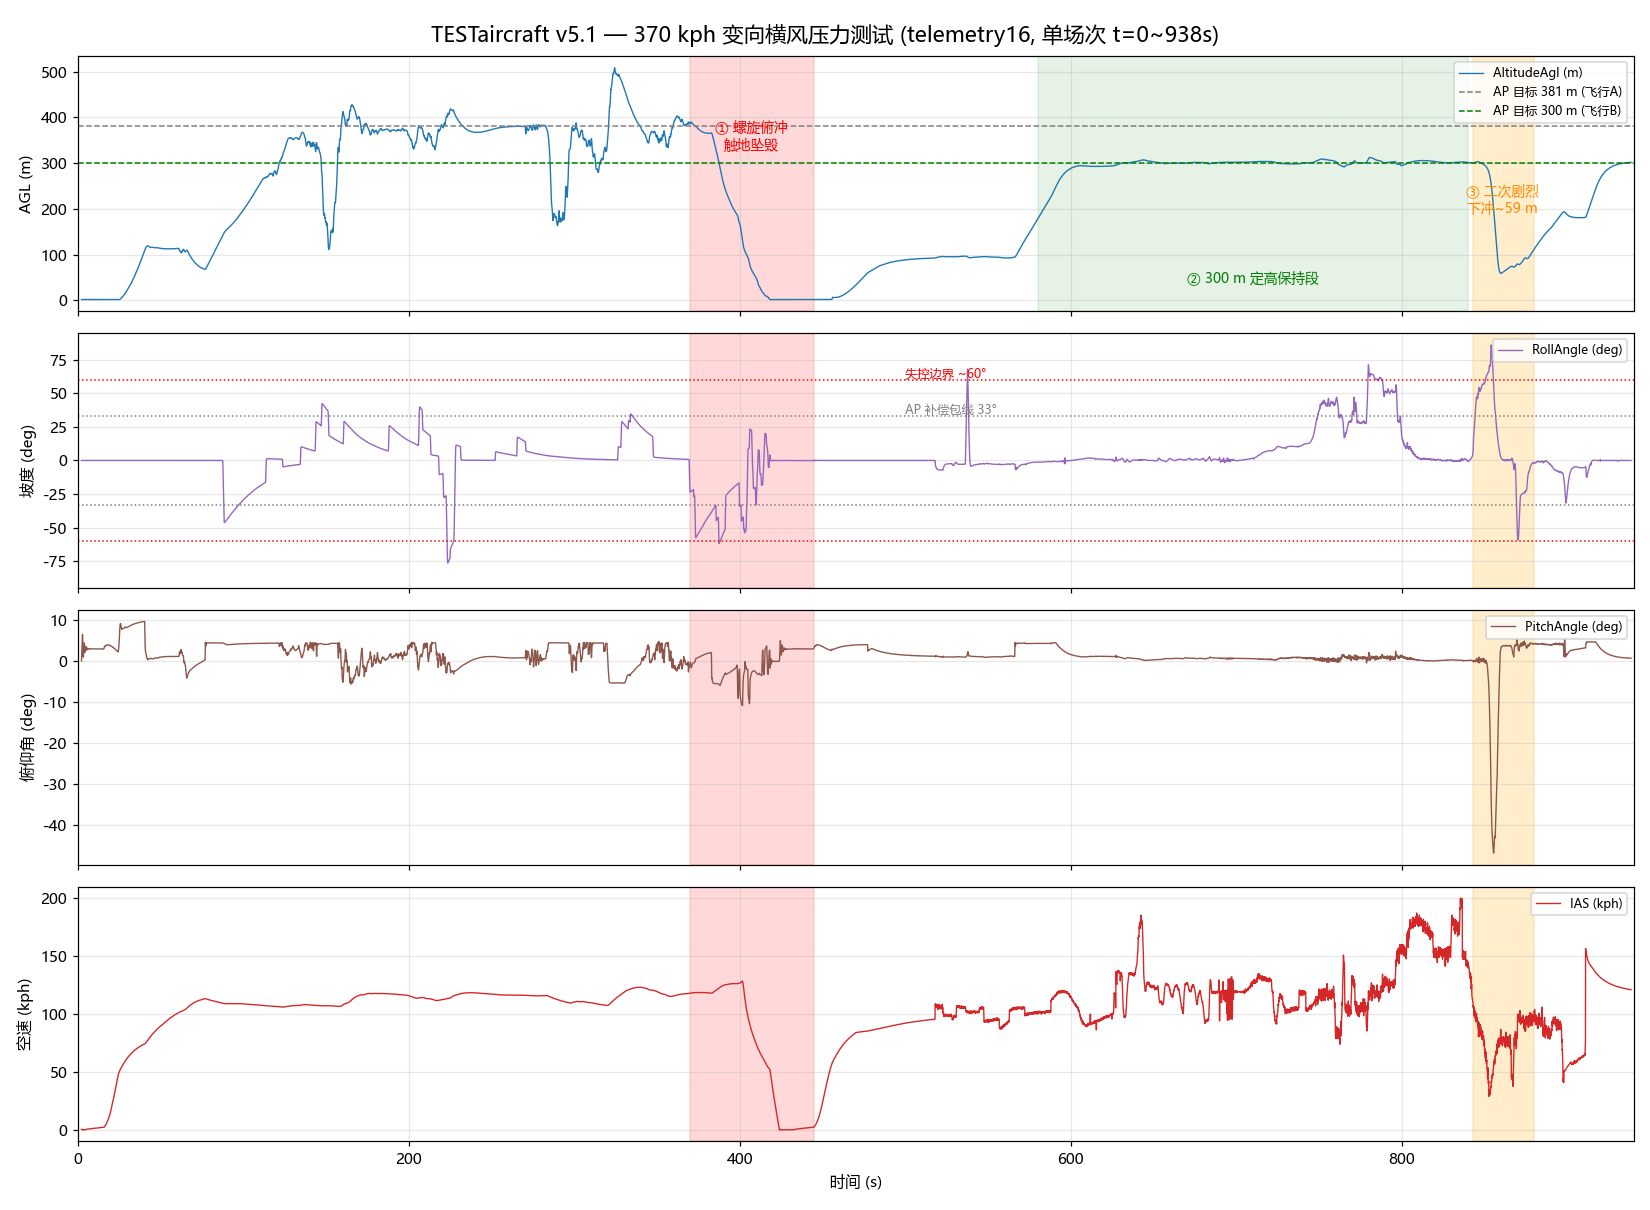
\includegraphics[width=\textwidth]{crosswind-stress-report.png}
\caption{370 km/h 变向横风压力测试全程曲线（单场次 938 s）：高度、坡度、俯仰角与空速}
\end{figure}
复核（图 1）表明：在目标 300 m 的保持段内（t=580--840 s），验证机在坡度反复达 $45^\circ$--$65^\circ$、空速 74--200 m/s 扰动的条件下将高度钉在 301--302 m，俯仰角速率均方根 0.1--0.5$^\circ$/s，垂直通道抗风性能确认合格。
测试中的地面接触事件（t$\approx$413--445 s）经操作者证词与数据联合判定为撞山：坠机段俯仰角始终维持低头 $-2^\circ$ 至 $-6^\circ$，与 AP 在线时应有的满舵抬头指令相悖，说明当时 AP 已断开，属手动飞行中的地形事件。该事件直接引出本报告的改型动机——AGL 定高模式对前方上升地形无前瞻能力。经复核修正：v5.1 峰值爬升约 10 m/s，在 103 m/s 地速下仅能跟随约 $6^\circ$ 缓坡，此类条件对无前瞻的 AGL 回路不可解。

\section{改型设计}
\subsection{地形前瞻模块（v6）}
受限于脚本沙箱无地形射线接口，采用沿航迹的一阶斜率外推：以 0.5 Hz 低通分别估计垂直速率 $\dot h$ 与无线电高度变化率 $\dot z$，地形抬升率 $\hat\tau=\mathrm{LPF}_{0.25}(\dot h-\dot z)$，前瞻最低高度
\begin{equation}
h_{\min}=60+\max(0,\hat\tau)\cdot L/V_g,\qquad L=200\ \mathrm{m},
\end{equation}
AP 有效目标取 $\max(h_{\text{set}},h_{\min})$；AP 断开时降级为告警（GPWS 简化式）。该方法的已知边界为：对连续缓坡有效，对悬崖状地形与转弯进入的新地形无预告能力。
\subsection{机动包线扩展（v6.1）}
应操作者要求将高度变化率上限由约 10 m/s 提升至 40 m/s，实现为三项耦合改动：指令限幅 $\theta_{\max}=\min\!\big(20^\circ,\arcsin(40/V_g)\big)$；失速保护（IAS $<75$ m/s 时抬头指令限 $+8^\circ$）；油门能量管理（IAS 越出 90--140 m/s 死区时以 0.4 s$^{-1}$ 速率自动收放）。
\subsection{控制仲裁特性（平台发现）}
遥测证实：脚本轴接管期间物理俯仰杆完全无效（AP 独占该轴），而配平轴不被接管且经舵面表达式 $u=\text{Trim}+\text{PID}(\cdots)$ 混入舵量。因此飞行员在不脱开 AP 的条件下仍持有配平超控通道，等效于真实电传的"超控不脱开"设计。该特性成为后文成绩归属判定的依据。

\section{验证试飞结果}
\subsection{包线验证（telemetry17）}
\begin{figure}[htbp]\centering
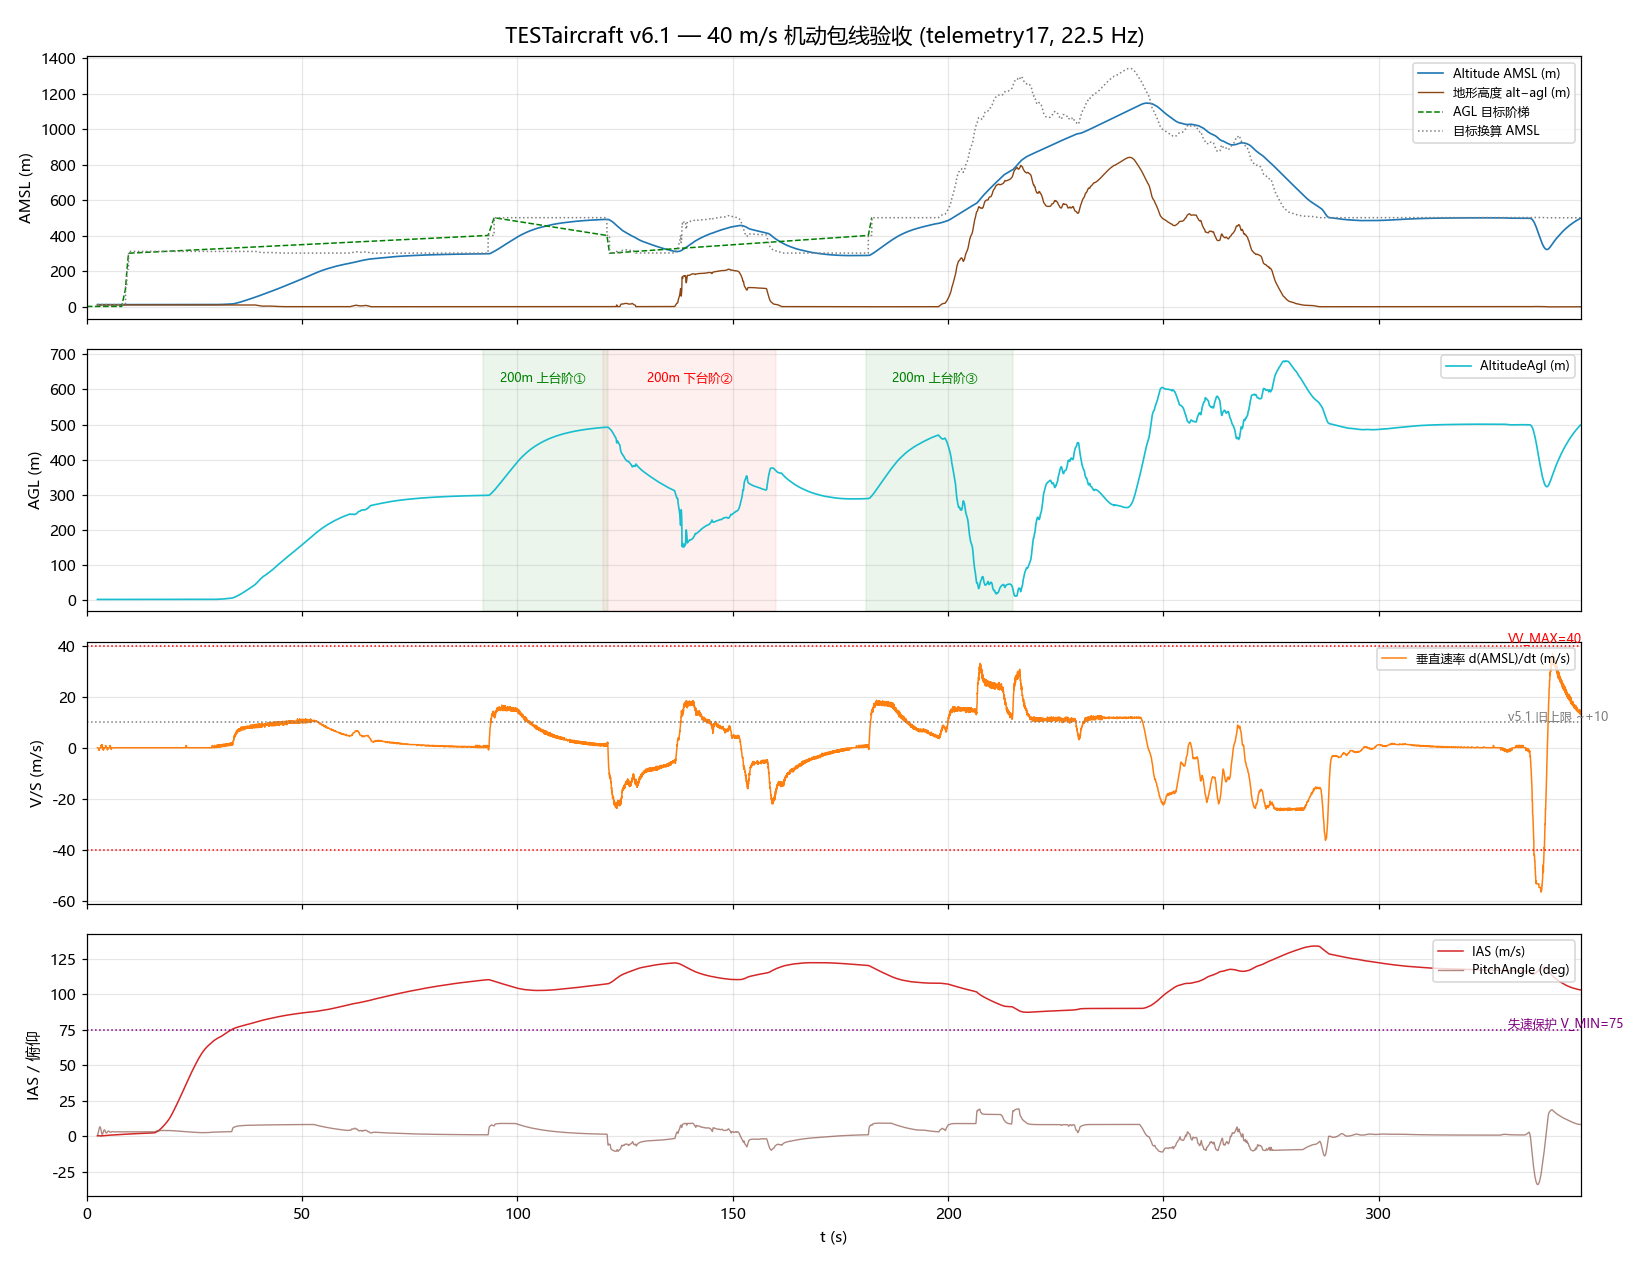
\includegraphics[width=\textwidth]{v61-envelope-report.png}
\caption{v6.1 机动包线验收：三次 200 m 台阶、地形 0--850 m 穿越}
\end{figure}
初判峰值爬升 39 m/s 经操作者驳回并复核改判：争议段舵面指令 47\% 时间满偏、姿态远超 AP 收敛特征，结合配平超控通道判定为手动（trim）注入成绩，AP 自主持续爬升实测 10--15 m/s。限幅机制本身确认工作（见 4.2 实弹数据）。油门能量管理三次试飞均未触发（油门由操作者管理），列为遗留验证项。
\subsection{前瞻实弹与馈出缺陷（telemetry18）}
\begin{figure}[htbp]\centering
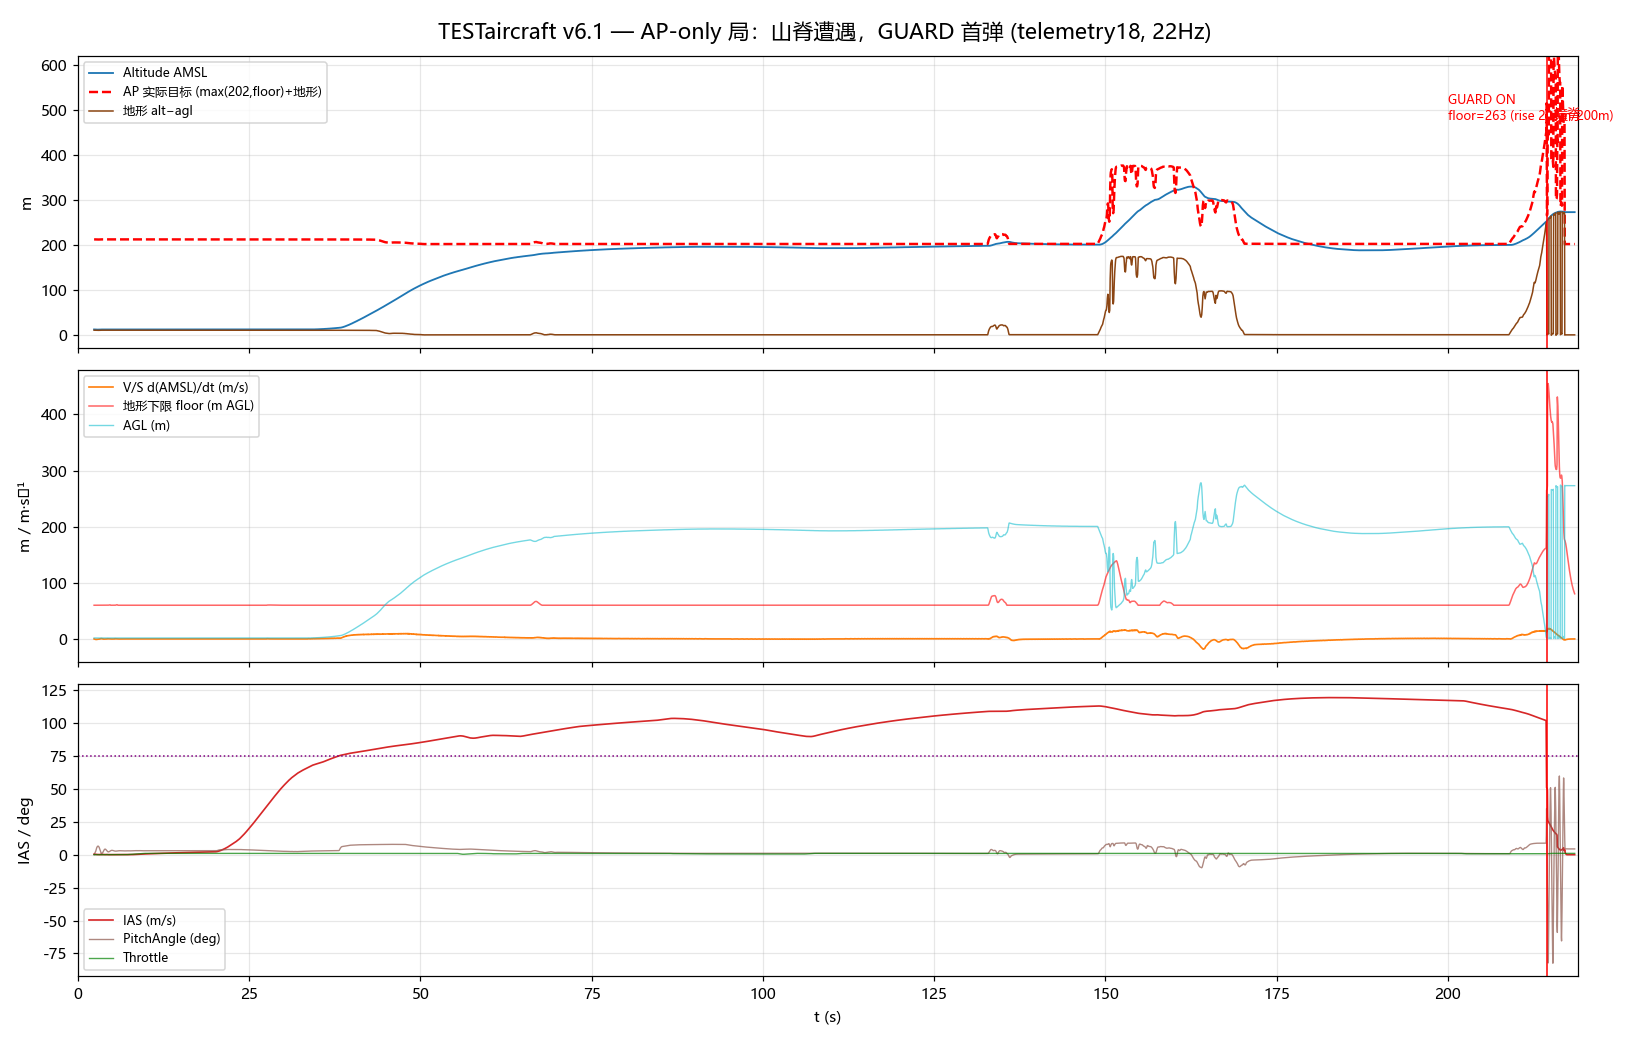
\includegraphics[width=\textwidth]{v61-guard-report.png}
\caption{GUARD 首次实弹触发（t=214.4 s，floor=263 m）与山脊接触过程}
\end{figure}
操作者以受控方式冲向一陡峻山脊。GUARD 于 t=214.4 s 正确报出 $h_{\min}=263$ m（外推抬升 203 m/200 m），AP 随即进入饱和：高度误差 167 m 对应指令需求约 $35^\circ$，被 $20^\circ$ 限幅截断，舵面 94\% 时间满偏，垂直速率 4 s 内由 +4.8 增至 +21.2 m/s。接触发生于报信后 1.4 s——地形沿迹抬升率约 47 m/s，超出机体爬升能力约 3 倍，属预告盲区内的不可避事件，与设计声明一致。
本次复盘识别出一项真实缺陷：爬升率前馈原采用 AGL 变化率，山区被地形运动污染（越脊背风侧将误指令低头）。v6.2 已改用 AMSL 速率（平地等价、山区正确）。
\subsection{AP 自主翻脊（telemetry19）}
\begin{figure}[htbp]\centering
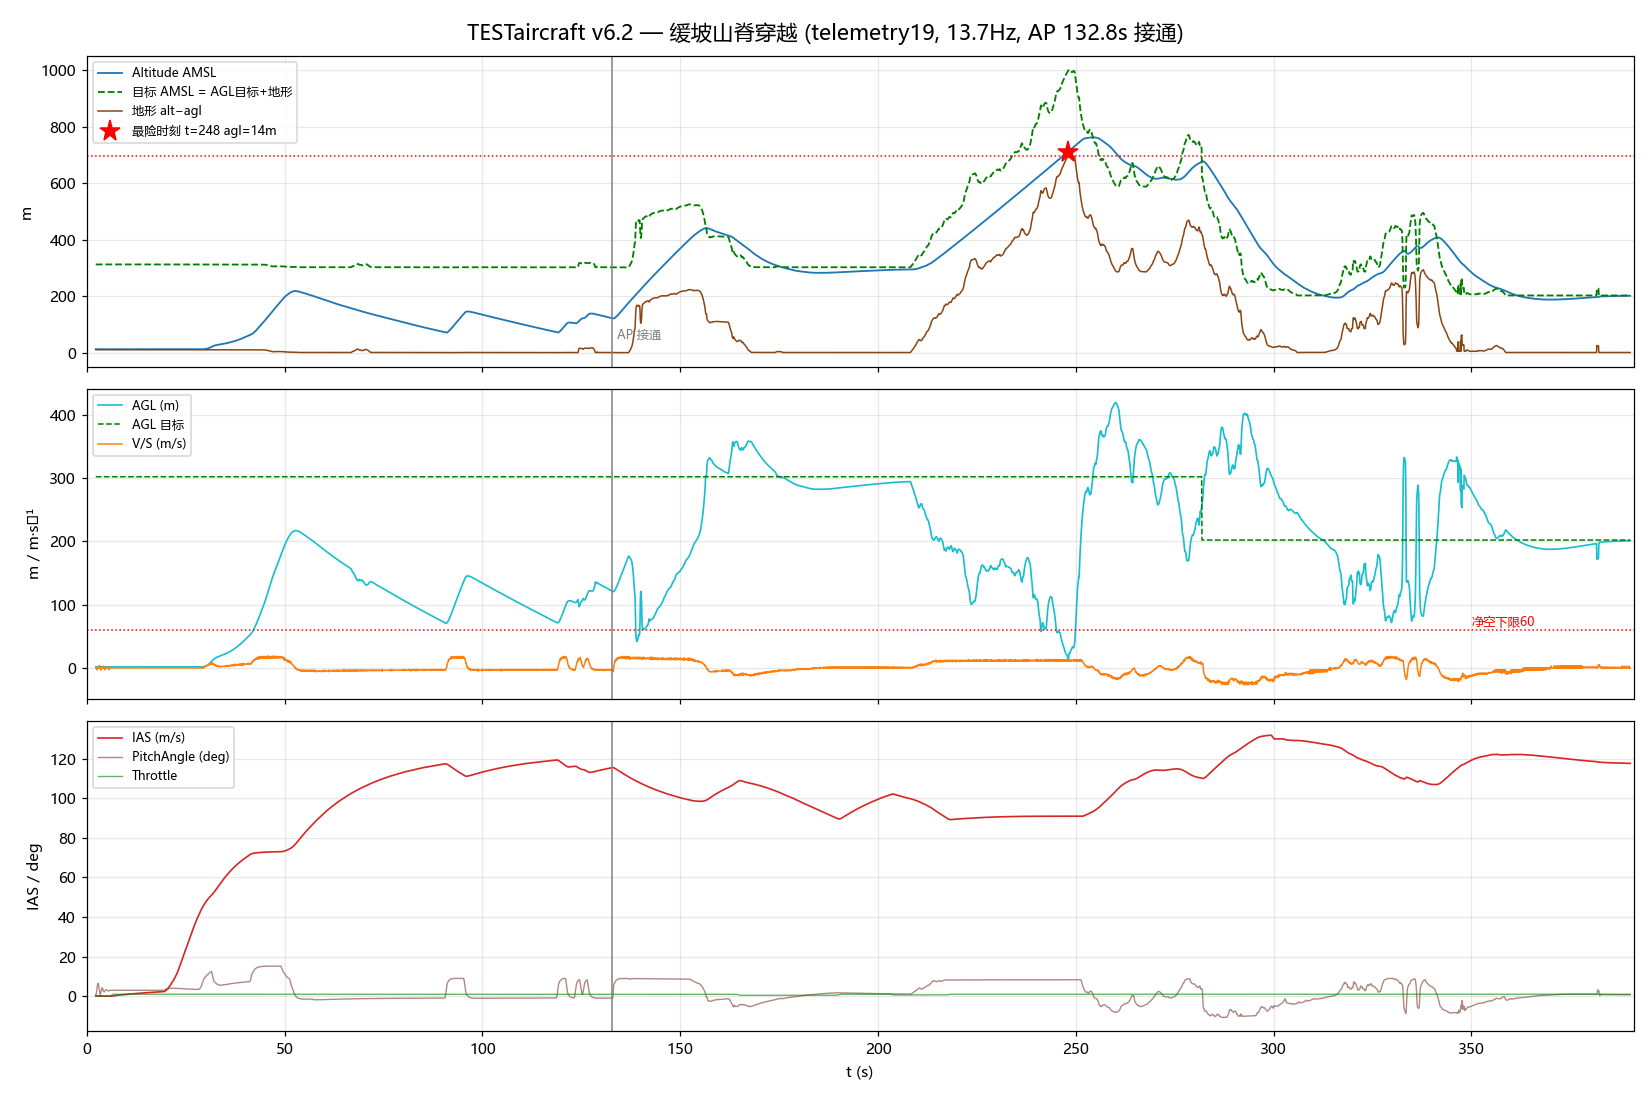
\includegraphics[width=\textwidth]{v62-ridge-report.png}
\caption{v6.2 回归局：AP-only 翻越 698 m 缓坡山脊，最小间隙 14 m}
\end{figure}
缓坡地形（沿迹抬升约 23 m/s）、操作者仅管理油门的条件下，AP 自主翻越 698 m 山脊，最小离地间隙 14 m（t=248 s），背风侧无异常低头，v6.2 修复回归通过。本局给出一项重要的包线修正：误差 288 m 时指令已顶 $20^\circ$ 限幅，但 IAS 90--115 m/s 下姿态实测最高约 $9^\circ$——\textbf{高速段真实上限为升降舵权限而非指令限幅}，$20^\circ$ 包线仅在低速段兑现。吃高度的机理为能量约束（地形抬升率 $>$ 持续爬升率），非控制律缺陷。
此外，告警逻辑经 v6.3 增加地面门（AGL $>3$ m；脚本代理白名单经穷举确认无接地标志，而地面态 AGL 恒读 1.6--2.0 m，判据两侧无歧义）。

\section{结论}
\begin{enumerate}
\item v6 系列改型全部验证项目通过：地形前瞻按设计边界工作（缓坡有效、悬崖属预告盲区），机动包线机制（限幅、失速保护）实弹确认，v6.2/v6.3 两项缺陷修复回归通过。课题以"飞控合格"收口。
\item 平台级新认知三项：配平轴构成天然的不脱开超控通道；高速段姿态能力受舵量权限（约 $9^\circ$@100 m/s）而非控制律限制；脚本接口速度量为 m/s。
\item 机体能力账本更新：持续爬升 10--15 m/s（推力受限）、瞬时可交换至约 21 m/s（动能交换）、可跟地形坡度上限约 $6^\circ$@100 m/s。
\item 遗留项：油门能量管理未获触发验证；滚转阻尼律（可选）未实施。
\end{enumerate}

\section{后续工作}
下一课题定为高性能验证机平台的目标追击/地形跟随方向：以机动性为第一设计约束（高推重比、大舵量），将滚转/偏航通道纳入脚本全权限控制，研究比例导引或纯追踪追击律在该平台上的实现与验证。

\end{document}
